\section{Introduction}

Глава посвящена преобразованиям Фурье, некоторым их свойствам и ключевым применениям в теории обработки сигналов. В частности, рассматриваются приложения в задачах фильтрации одномерных и двумерных сигналов, Фурье-спектроскопии, формировании признакового описания входного сигнала.

\section{References Review}

\begin{itemize}
    \item ~\cite{MITcourse} -- открытый курс MIT, отдельные лекции которого посвящены преобразованиям Фурье и их приложениям в анализе сигналов;
    \item ~\cite{GonzalezWoods} -- источник, содержащий информацию об анализе и обработке изображений, в частности о применении преобразования Фурье для фильтрации изображений;
    \item ~\cite{LiDAR1, LiDAR2} -- работы, описывающее применение преобразования Фурье к сигналу LiDAR для построения признакового описания объекта;
\end{itemize}

\section{Main Part}

\subsection{Связь преобразований Фурье с рядом Фурье}

Для того, чтобы ввести преобразование Фурье, предлагается рассмотреть ряд Фурье для апериодической функции как предел ее периодического обобщения, тем самым на простом примере показать связь преобразования Фурье с рядами Фурье. Это рассуждение не является строгим доказательством, а лишь некоторой интуицией о связи понятий.

Здесь и далее сигнал понимается математически как функция одной или нескольких независимых величин.

Известно, что любой периодический сигнал может быть представлен в виде своего ряда Фурье. 
Теперь же рассмотрим некоторый апериодический сигнал, например, простой импульс $x(t) = \mathbb{I}(t \in [-S, S])$. 
\begin{figure}[!htb]
\center{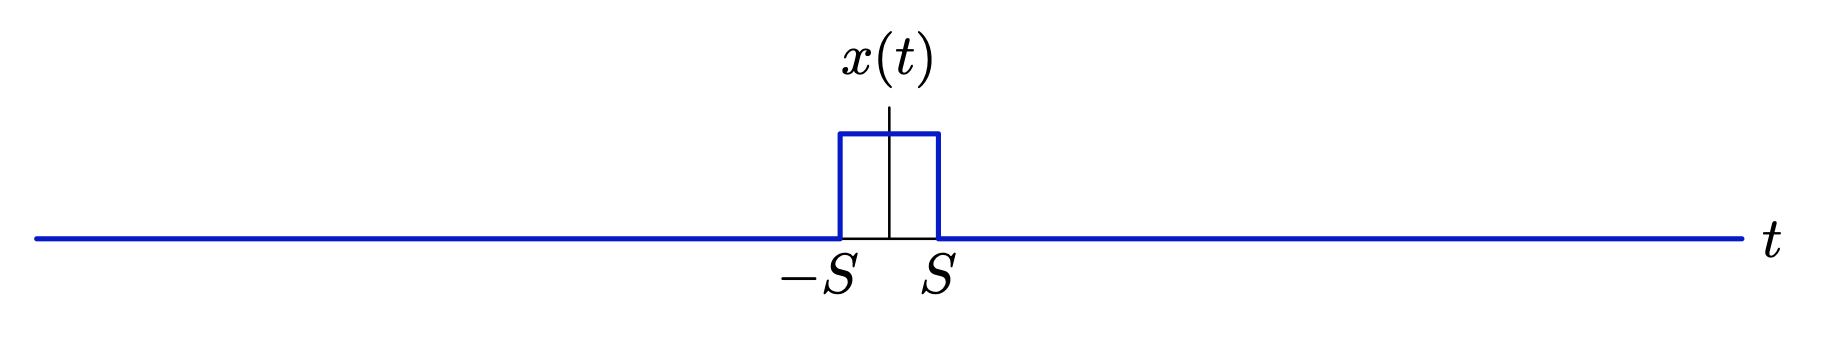
\includegraphics[width=0.7\textwidth]{chapters/grigorev_s1/pictures/xt}}
\caption{Апериодический сигнал $x(t)$}
\end{figure}

Апериодический сигнал может рассматриваться как периодический с бесконечным периодом.
Видоизменим сигнал $x(t)$, сделав его переодическим, просто сдвигая импульс на значение периода и суммируя:
$$x_T(t) = \sum \limits _{k=-\infty}^{\infty} x(t+kT) .$$
\begin{figure}[!htb]
\center{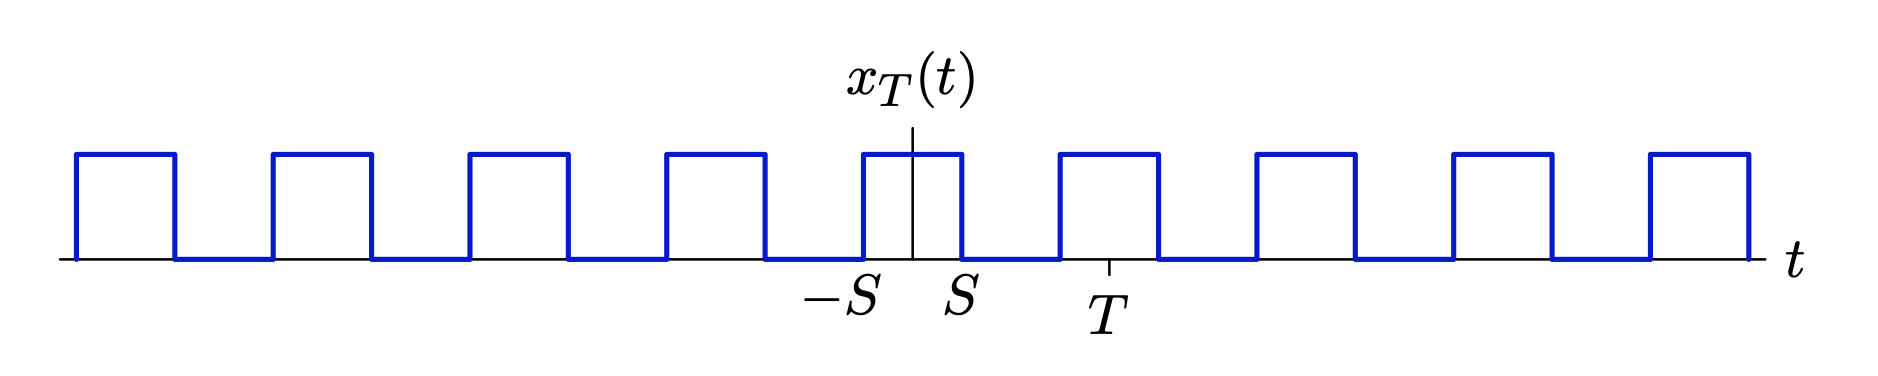
\includegraphics[width=0.7\textwidth]{chapters/grigorev_s1/pictures/xtt}}
\caption{Периодический обобщение $x_T(t)$ исходного сигнала $x(t)$}
\end{figure}

Сигнал, очевидно, периодический и, более того, предел такого периодического обобщения при $T\to \infty$ равен исходному сигналу:
$$x(t) = \lim \limits _{T \to \infty} x_T(t).$$

Дальнейшая идея состоит в том, чтобы попробовать разложить в ряд Фурье периодическое обобщение $x_T(t)$ исходного сигнала и перейти к пределу по $T$ для того, чтобы сделать некоторые выводы о таком преобразовании.

Периодическое обобщение $x_T(t)$ раскладывается в ряд Фурье, коэффициенты ряда Фурье для периодического сигнала выглядят следующим образом:
$$a_k = \frac{1}{T} \int \limits_{-T/2}^{T/2} x_T(t) e^{-i \frac{2\pi}{T}kt} dt = \frac{1}{T} \int \limits_{-S}^{S} e^{-i \frac{2\pi}{T}kt} dt = \frac{2}{T} \frac{\sin(\omega S)}{\omega}.$$
\begin{figure}[!htb]
\center{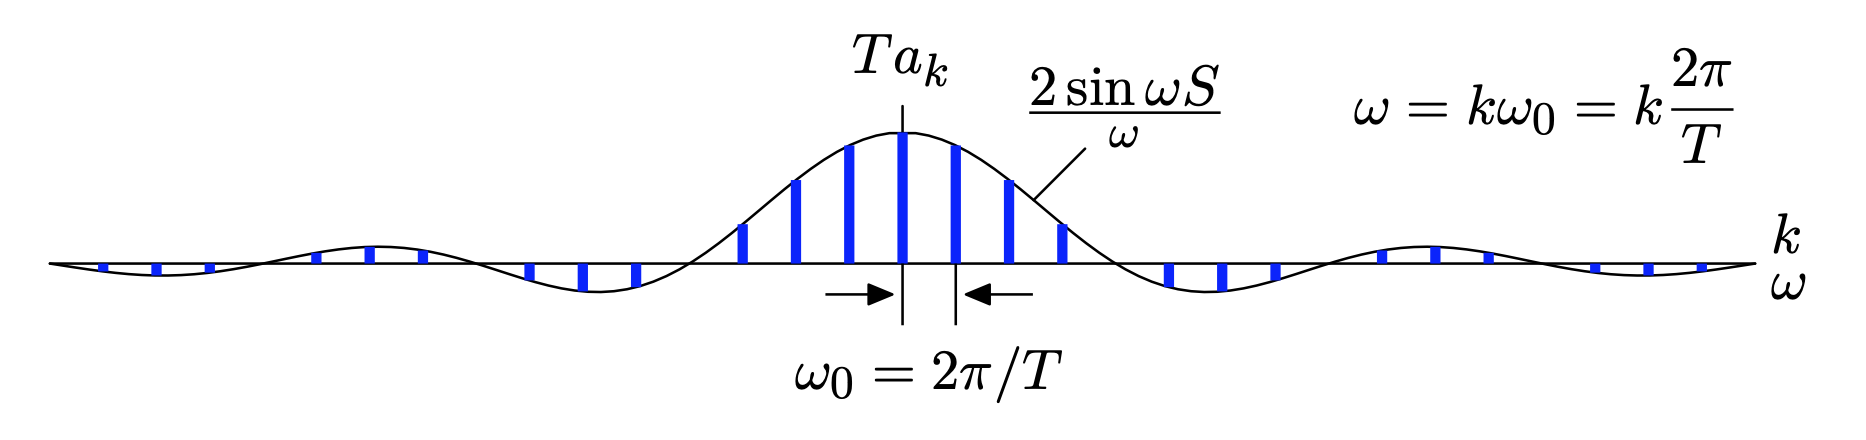
\includegraphics[width=0.7\textwidth]{chapters/grigorev_s1/pictures/tak}}
\caption{График зависимости $T a_k = f(k)$ и профиль амплитуд $E(\omega)$}
\end{figure}

Рассмотрим зависимость коэффициентов Фурье, масштабированных на значение периода, как функцию от номера $k$. Заметим, что увеличение периода вдвое приводит к тому, что огибающая не изменяется, но число коэффициентов, находящихся в заданном интервале частот $\omega$, увеличится вдвое. И в пределе величина $T a_k$ стремится к непрерывной функции $E(\omega)$, которая описывает профиль амплитуд:
$$\lim \limits_{T\to \infty}T a_k = \lim \limits_{T\to \infty} \frac{1}{T} \int \limits_{-T/2}^{T/2} x(t) e^{-i \frac{2\pi}{T}kt} dt = \frac{2}{T} \frac{\sin(\omega S)}{\omega} = E(\omega).$$
Причем функции $E(\omega)$ не зависит от $T$.

В обратную сторону, используя предельный переход к разложению периодического сигнала в ряд Фурье, можно получить представление исходного сигнала через интеграл от функции $E(\omega)$, домноженной на комплексный вес:
\begin{align*} 
x(t) & = \lim \limits _{T \to \infty} x_T(t) = \lim \limits _{T \to \infty} \sum \limits_{k=-\infty}^{\infty} \frac{1}{T} E(\omega) E^{i \frac{2 \pi}{T}kt} = \\
& =  \lim \limits _{T \to \infty} \sum \limits_{k=-\infty}^{\infty} \frac{\omega_0}{2 \pi} E(\omega) E^{i \omega t} = \frac{1}{2 \pi} \int \limits_{-\infty}^{\infty} E(\omega) e^{i \omega t} d \omega.
\end{align*}
Сумма здесь перешла в интеграл в Римановском плане. Таким образом, для простого сигнала получили преобразование Фурье. Проделанное не является выводом преобразования, а лишь описывает некоторую интуицию о связи ряда Фурье и преобразования Фурье.

\subsection{Преобразования Фурье}

Преобразование Фурье в общем случае имеет следующий вид:
$$X(i \omega) = \int \limits_{-\infty}^{\infty} x(t) e^{-i\omega t} dt.$$
Преобразование обратимо, обратное выглядит в меру симметрично:
$$x(t) = \frac{1}{2\pi} \int \limits_{-\infty}^{\infty} X(i \omega) e^{i \omega t} d\omega.$$
Преобразование Фурье обладает следующими характерными свойствами:
\begin{enumerate}
\item линейность: $a \, x_1(t) + b \, x_2(t) = a\,X_1(i \omega) + b\,X_2(i \omega)$;
\item сдвиг времени: $x(t - t_0) = e^{- i \omega t_0} X(i \omega)$;
\item масштабирование времени: $x(at) = \frac{1}{|a|}X(\frac{i \omega}{a})$;
\item дифференцирование: $\frac{dx(t)}{dt} = i \omega X(i \omega)$;
\end{enumerate}

\subsection{Дискретные преобразования Фурье}

На практике часто приходится иметь дело с сигналами, которые известны в конечном наборе точек $t \in [0, N-1]$, то есть дискретными. Будь это дискретность по времени или пространству не столь важно. Важно, чтобы шаг между точками, соответствующими наблюдаемым значениям, был равномерен.

Пусть $x(t) ~-$ исходный входной сигнал,  $t \in [0, N-1]$, $\{x_n\}_{n=0}^{N-1} ~-$ входной сигнал в дискретных временных точках $n=0,\dots,N-1$ c постоянным временем сэмплирования $dt=1$, то есть дискретный сигнал задает ступенчатую аппроксимацию $x(t)$.
Дискретное преобразования Фурье для данного сигнала можно получить из преобразования Фурье для функции, расписывая его для описанной дискретной аппроксимации, то есть для $N$ ступенек ширины $1$ с высотой, задаваемой дискретным сигналом:
\begin{align*}  
& X(i \omega) = \int \limits_{\infty}^{\infty} x(t) e^{-i\omega t} dt = \int \limits_{0}^{N-1} x(t) e^{-i\omega t} dt = \sum \limits _{n=0}^{N-1} x_n e^{-i \omega n},\\
& \omega=k \frac{2 \pi}{N}, \, k=0,\dots,N-1.
\end{align*}
Набор частот в данном случае определяется следующим образом. Очевидно, что число частот равно числу входных значений, чтобы на выходе размерность сохранялась. Остается заметить, что исходная дискретная аппроксимация задана на отрезке $[0, N]$ и может быть периодически продлена на оставшуюся ось с периодом $N$. Вспоминая о связи ряда Фурье и преобразования Фурье, получим набор частот $\omega=k \frac{2 \pi}{N}, \, k=0,\dots,N-1$. Данный набор частот может быть выбран иначе, например, симметрично относительно $0$ согласно формуле Эйлера.
Общий вид прямого и обратного дискретных преобразований Фурье выглядит следующим образом. Прямое дискретное преобразование Фурье \textit{(DFT)}: 
$$X_k = \sum \limits _{n=0}^{N-1} x_n e^{-i\frac{2 \pi}{N}kn}$$,
обратное дискретное преобразование Фурье \textit{(IDFT)}:
$$x_n = \frac{1}{N} \sum \limits _{k=0}^{N-1} X_k e^{i\frac{2 \pi}{N}kn}.$$ 

Заметим, что дискретное преобразование Фурье можно представить в матричном виде. Исходный дискретный сигнал запишется в виде столбца, коэффициенты из комплексных экспонент образуют матрицу. Преобразование — умножение матрицы на столбец, то есть $N^2$ операций умножения.  Тогда сложность, соответствующая наивному алгоритму равна $O(N^2)$. Существует более эффективный алгоритм со сложностью $O(N \log N)$, принимающий во внимание структуру задачи. Данный алгоритм известен как быстрое преобразование Фурье. Алгоритмы синонимичны, зачастую когда говорят, что используется DFT, то подразумевается вычисление именно FFT.

Далее будут упомянуты некоторые приложения преобразований Фурье в анализе сигналов. 

\subsection{Фурье фильтрация}

Пожалуй, одно из основных применений преобразования Фурье — это фильтрация сигнала. Зачастую шум, который мы хотим отфильтровать от исходного сигнала, представляет собой высокочастотные или низкочастотное колебания. Очевидно, что наиболее удобно в данном случае производить фильтрацию сигнала по частотному спектру. Общая процедура заключается в применении преобразования Фурье к исходному сигнала $x(t)$, наложению фильтра $H(\omega)$ на выделенный спектр $X(\omega)$ и применении обратного преобразования Фурье для получения отфильтрованного сигнала $y(t)$.
\begin{figure}[!htb]
\centering
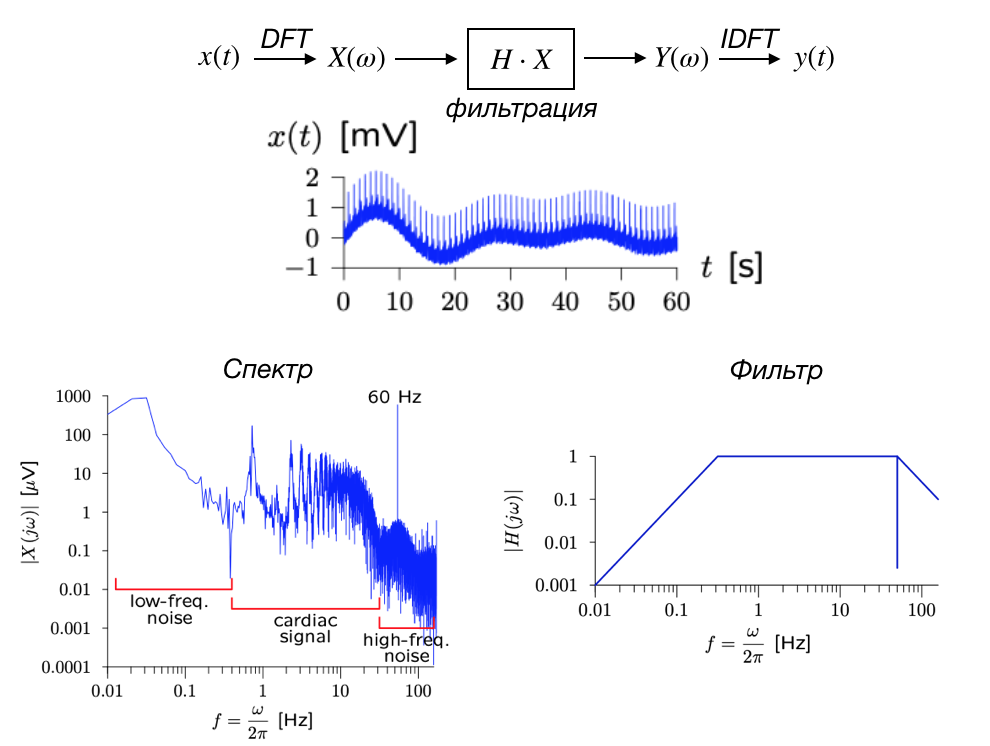
\includegraphics[width=16cm]{chapters/grigorev_s1/pictures/s6}%
\caption{Схема фильтрации электрокардиограммы}
\end{figure}

Растровое изображение тоже является сигналом как функция яркости $f(x, y)$ от координат пикселя $x=0,\dots,N-1$, $y=0,\dots,N-1$. Зачастую изображения содержат периодический высокочастотный шум, который требуется отфильтровать.

Двумерное преобразование Фурье выглядит следующим образом:
$$F(\omega_x, \omega_y) = \sum \limits _{x=0}^{N-1} \sum \limits _{y=0}^{N-1} f(x, y) e^{-i (\omega_x x + \omega_y y)}.$$
Частоты $\omega_x$ и $\omega_y$ определяются аналогично одномерному случаю, таким образом, они  принимают следующие $N$ значений:
$$\omega_x, \omega_y \in \left\{ k \frac{2 \pi}{N} \Bigg| k=0,\dots,N-1 \right\} .$$
На практике удобно сдвинуть часть частот на $2 \pi$, что допустимо по формуле Эйлера, сделав частоты симметричными по отношению к $0$ с шагом $\frac{2 \pi}{N}$.

Результат преобразование Фурье входного изображения представляет собой комплекснозначное изображение. Комплекснозначное изображение описывается амплитудами и фазами, как правило для фильтрации шума достаточно анализа изображения, соответствующего амплитудам спектра.
Таким образом, для частотного спектра производится фильтрация высокочастотных пиков амплитуд, соответствующих шуму и применяется обратное преобразование Фурье для получения отфильтрованной картинки.
\begin{figure}[!htb]
\centering
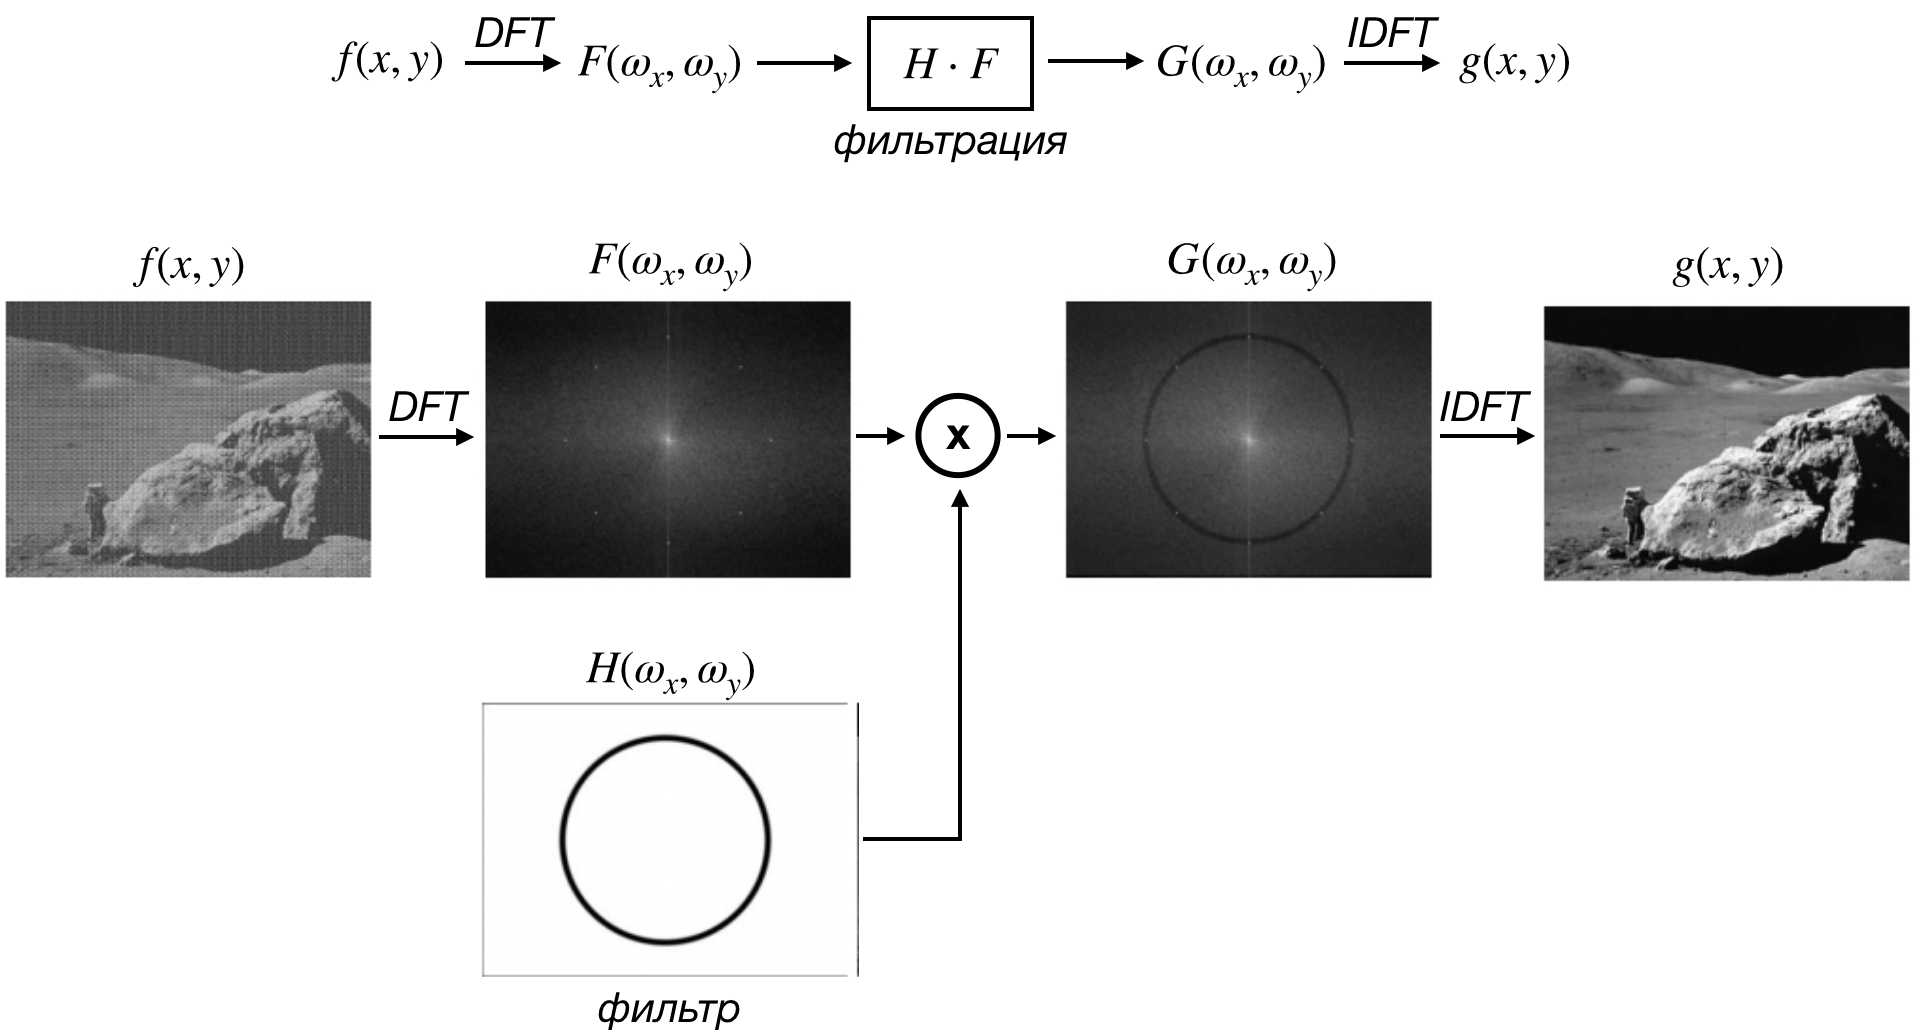
\includegraphics[width=16cm]{chapters/grigorev_s1/pictures/image_filtartion_with_scheme}%
\caption{Схема фильтрации изображения}
\end{figure}

\newpage
\subsection{Фурье спектроскопия}

Преобразование Фурье находит свои применения и в физике, в частности в оптике. Задача спектроскопии — определение спектра излучения некоторого источника, в общем случае немонохроматического.
Интерферометр Майкельсона $~-$ основа Фурье-спектроскопии, прибор позволяет определить спектр излучения по интерференционной картине.
\begin{figure}[!htb]
\centering
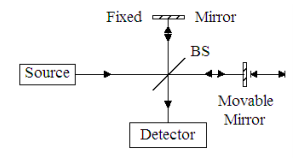
\includegraphics[width=8cm]{chapters/grigorev_s1/pictures/interferometer}%
\caption{Схема интерферометра Майкельсона}
\end{figure}
Здесь можно рассмотреть два случая — монохроматический и немонохроматический источник. В первом случае зависимость интенсивности от геометрической разности хода имеет следующий вид:
$$I(\delta) = \frac{1}{2} \left[ \cos\left( \frac{2 \pi \delta}{\lambda} \right) + 1 \right],$$ 
где $\delta ~-$ разность хода, $\lambda ~- $ длина волны. В данном случае параметр длины волны $\lambda$ находится аналитически, например, через первый минимум интенсивности.
В немонохроматическом случае суммируются интенсивности от всех длин волн:
$$I(\delta) = \sum \limits _j \frac{1}{2} \left[ \cos\left( \frac{2 \pi \delta}{\lambda_j} \right) + 1 \right],$$ 
аналитически спектр не найти. Однако в данном случае спектр излучения источника можно получить через преобразование Фурье полученной спектрограммы. 
\begin{figure}[!htb]
\centering
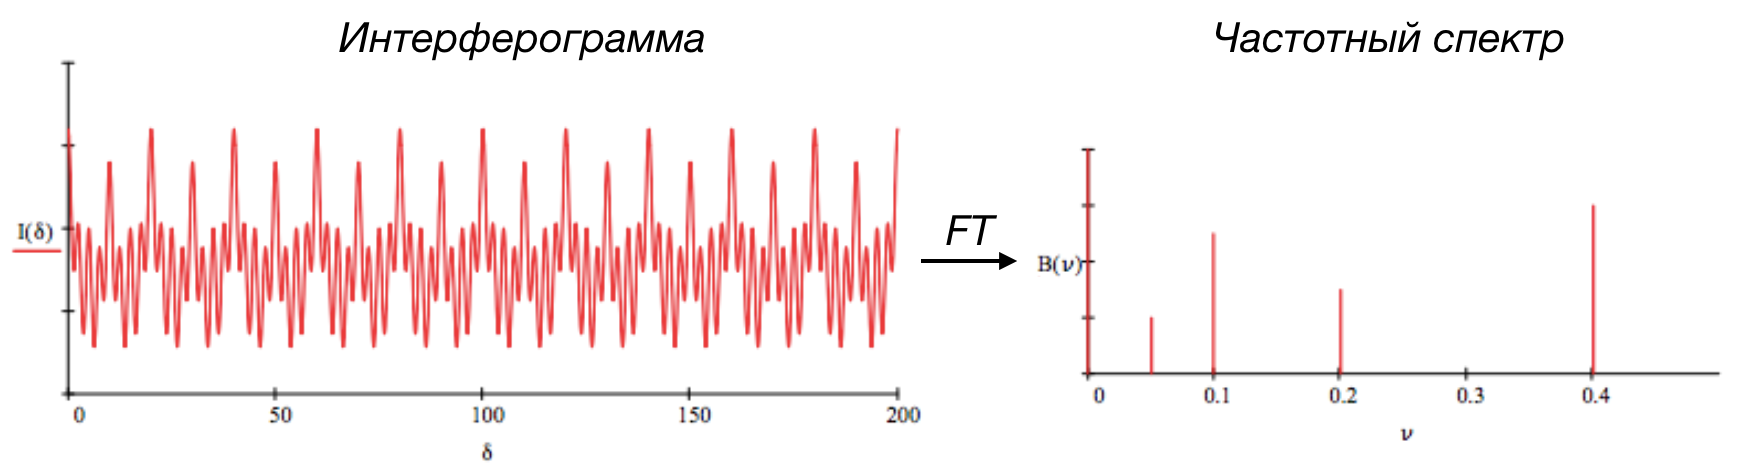
\includegraphics[width=14cm]{chapters/grigorev_s1/pictures/interferogram_spectrum}
\caption{Схема определения спектра излучения по интерферограмме}
\end{figure}

\subsection{Преобразования Фурье в LiDAR}

Последнее применение преобразование Фурье, которое будет освещено в данном семинаре, связано с построением признакового пространства в задачах, где исходные данные представляют собой временной ряд. Данное применение рассматривается на примере LiDAR, метода измерения расстояния до объекта. Базовый физический принцип прибора тривиален, расстояние вычисляется через время возврата волны (лазера) с известней скоростью распространения (скоростью света).
\begin{figure}[!tb]
\centering
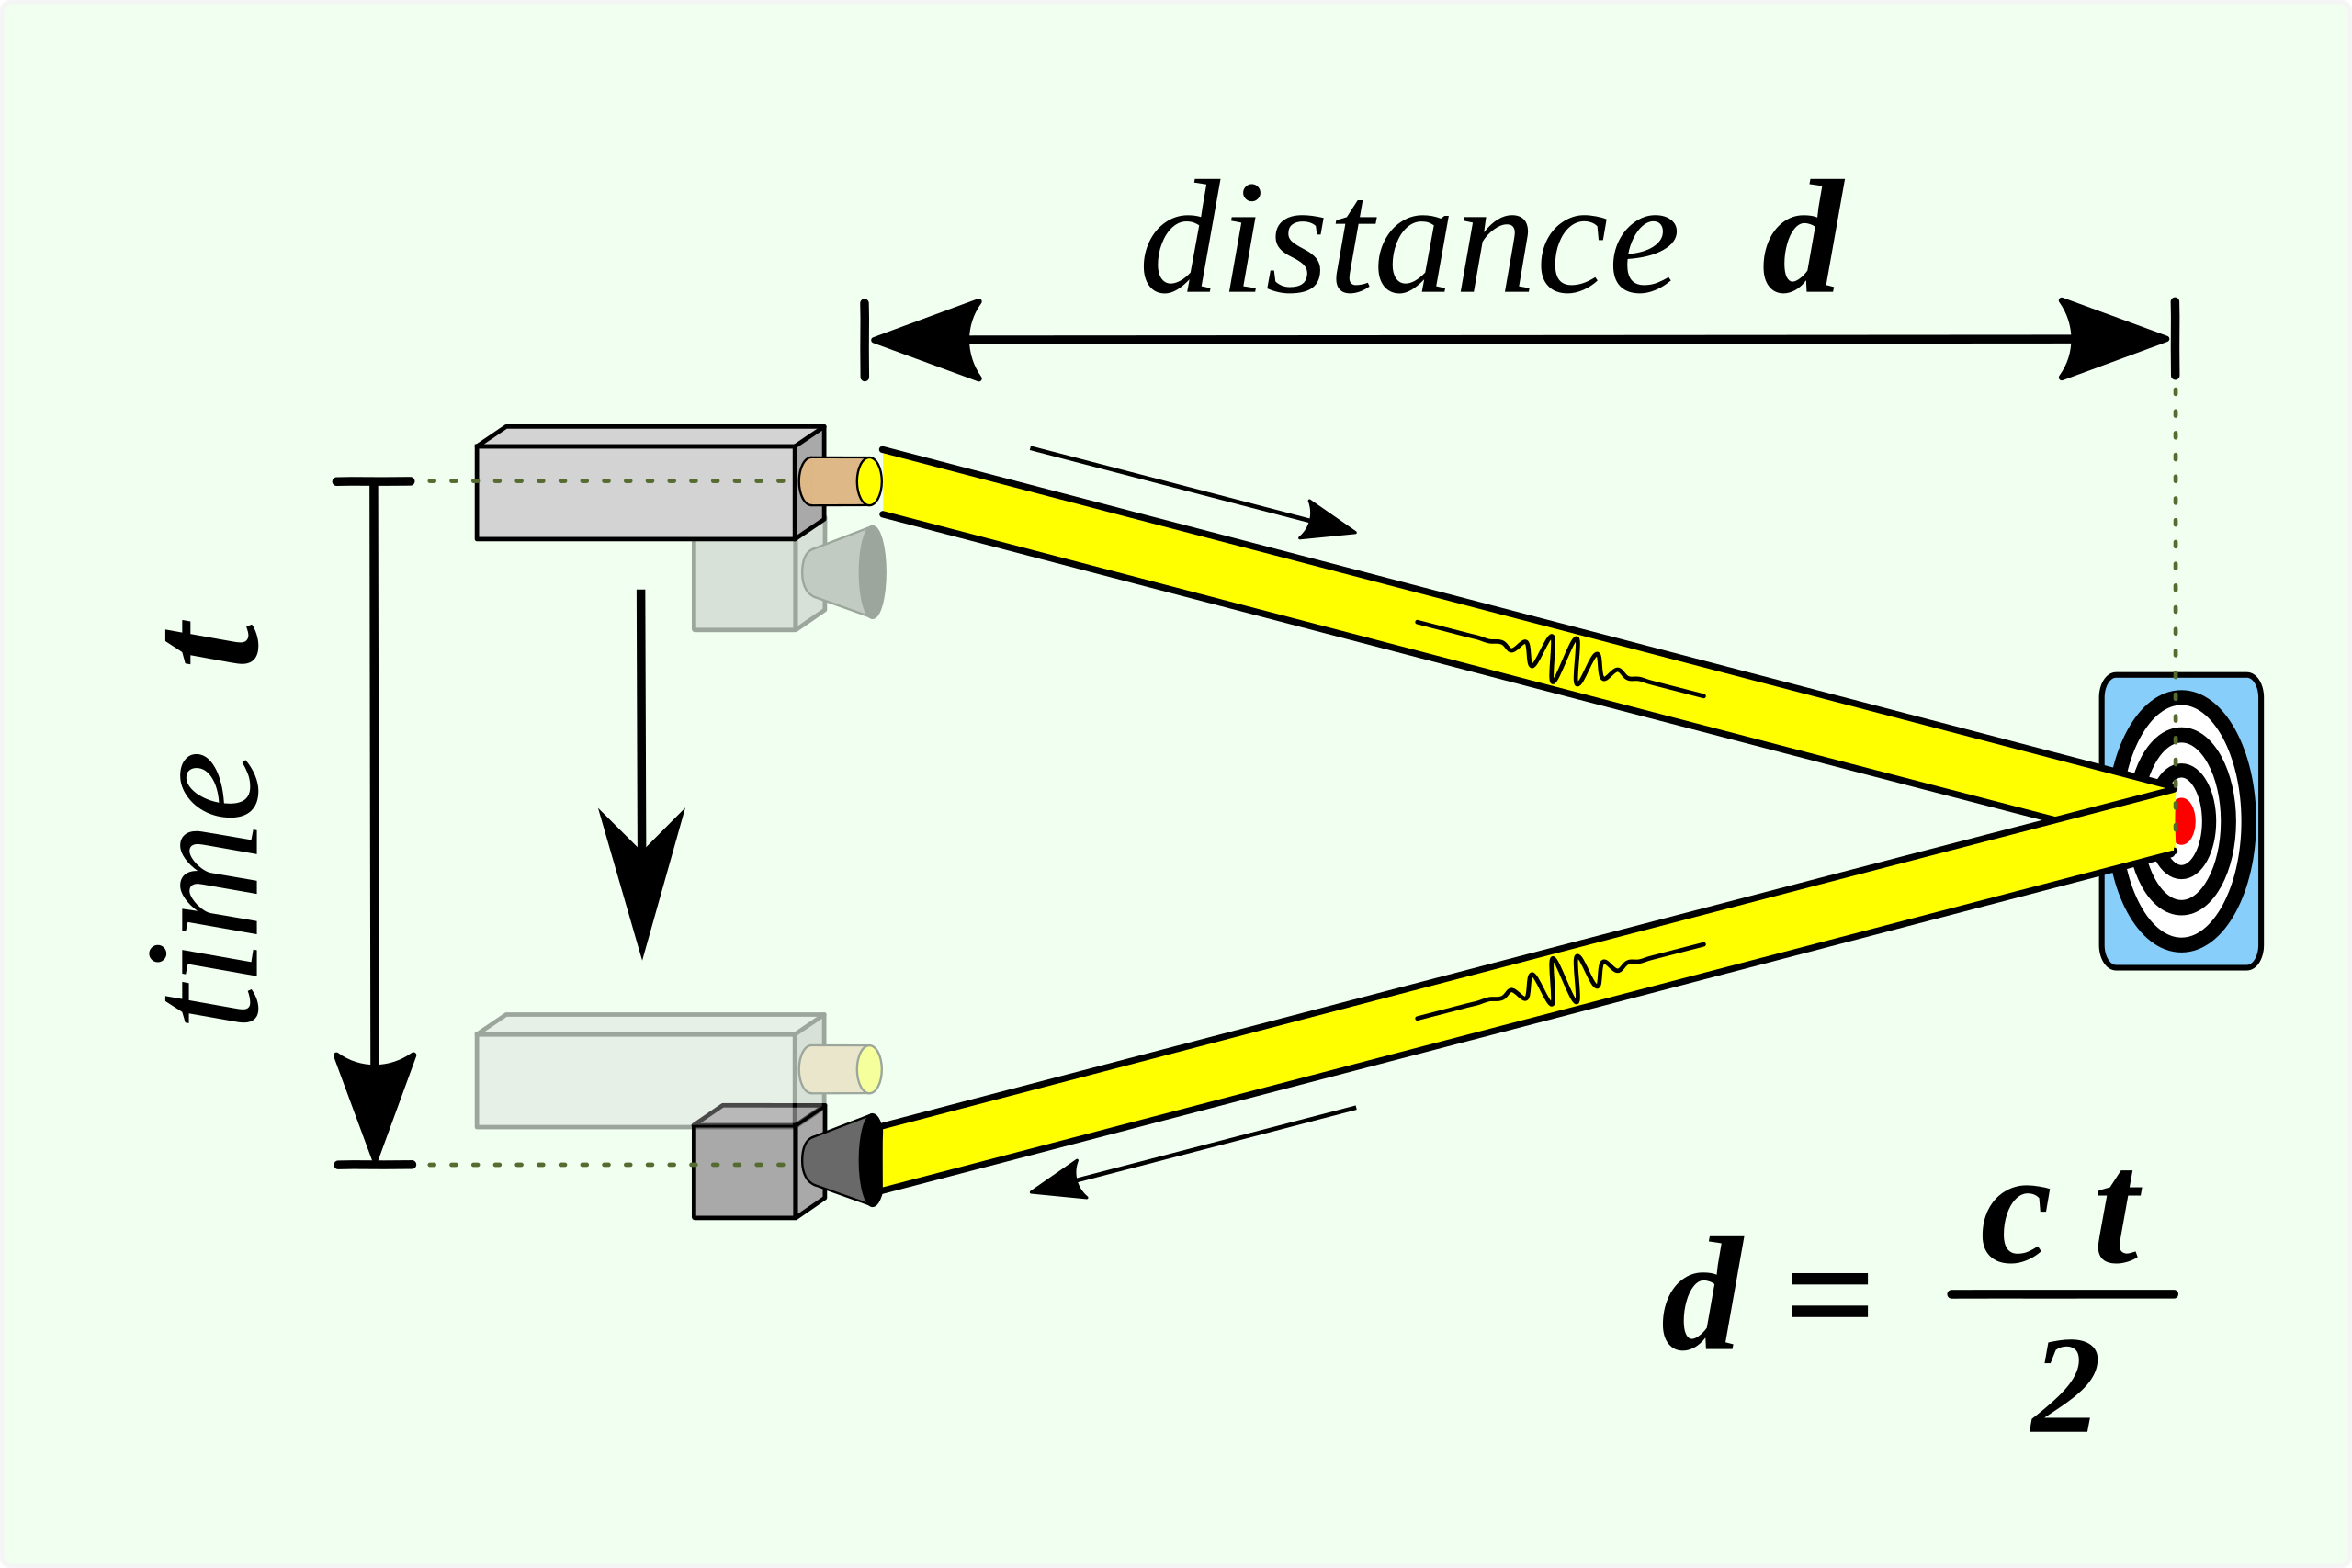
\includegraphics[width=6cm]{chapters/grigorev_s1/pictures/lidar_scheme}%
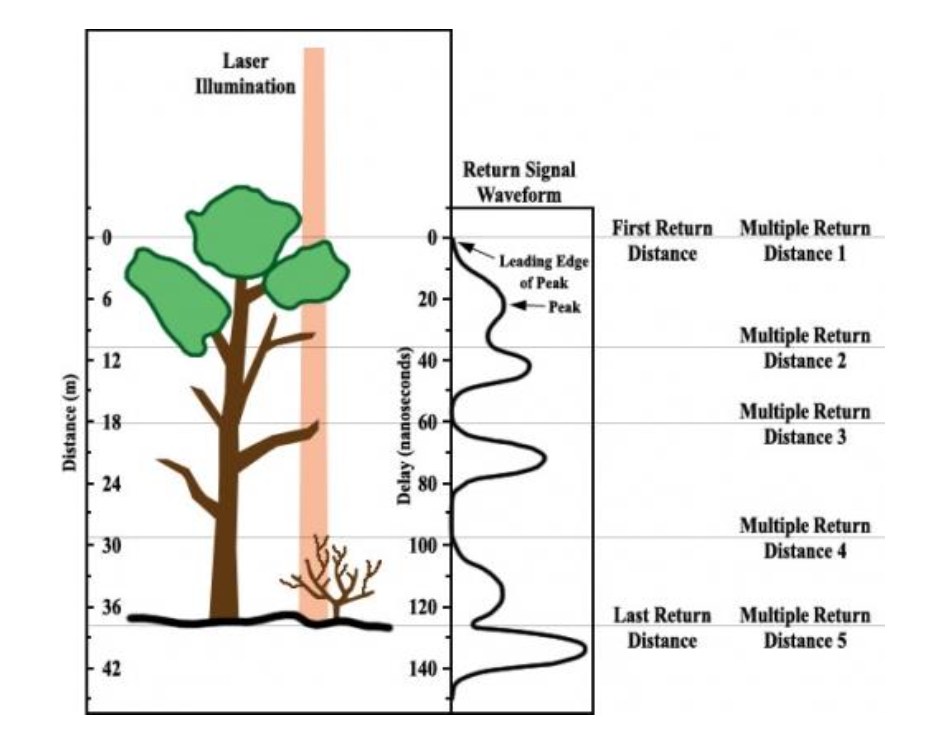
\includegraphics[width=6cm]{chapters/grigorev_s1/pictures/lidar}%
\caption{Схема LiDAR и регистрируемый сигнал}
\end{figure}

Как правило статьи, связанные с практическим применением LiDAR, имеют следующее применение преобразования Фурье вне зависимости от решаемой задачи машинного обучения. Применение состоит в формировании признакового пространства для алгоритма машинного обучения путем применения DFT к LiDAR сигналу. Объект — временной ряд $\{x_n\}_{n=0}^{N-1}$ амплитуд отраженного от поверхности сигнала. Для данного временного ряда вычисляется DFT, $\{X_k\}_{k=0}^{N-1} ~- $ сигнал после DFT, используемый в качестве признакового описания сигнала. В силу того, что данные величины комплекснозначны $\forall k = 0, \dots, N-1 \,\,\,\, X_k \in \mathbb{C}$, их удобно описывать через амплитуду и фазу соответственно. Остается уточнить, что для действительнозначного сигнала (а временной ряд амплитуд действительнозначен) использование всех значений, полученных в результате применения DFT, избыточно в силу свойства DFT для действительнозначного входного сигнала: $X_k = \overline{X_{N-k}} \,\, \forall k$. Таким образом, итоговое признаковое описание сигнала задается амплитудами и фазами половины значений DFT.

\section{Questions To Discussion}

\begin{enumerate}
\item В чем заключается логическая связь между рядами Фурье и преобразованием Фурье? 
\item Алгоритмическая сложность DFT и FFT?
\item Основное применение преобразование Фурье в анализе сигналов?
\item Чему соответствует центральная точка изображения, представляющего амплитуды образа DFT исходной картинки? 
\item Чему равна эффективная размерность признакового пространства, полученного применением DFT к действительнозначному временному ряду длины $T$, как формируется это признаковое пространство?
\end{enumerate}